\chapter{Objetivos del proyecto}

//TODO Cambiar visión general, no corresponde con la realidad

	\section{Visión general}

		En esta sección se pueden ver las distintas partes que componen el capítulo.

		\begin{itemize}
			\item \textbf{Visión general:}
				
			Definición del contenido del capítulo.
			
			\item \textbf{Definición del proyecto:}
				
			Establecimiento de los objetivos del proyecto y su alcance.

			\item \textbf{Producto final:}
				
			Descripción funcional del producto final.

			\item \textbf{Descripción de la realización:}
				
			Descripción del método de desarrollo que se ha utilizado, especificación de productos intermedios, todas las tareas del proyecto y su asociación con los perfiles del equipo incluyendo EDT.

			\item \textbf{Planificación:}
				
			Estimación de cargas por perfil y grafos para la representación de la planificación de tareas.

			\item \textbf{Presupuesto:}
				
			Definición del presupuesto necesario para la realización del proyecto.
		\end{itemize}

	\section{Definición del proyecto}

		\subsection{Objetivos}

			El objetivo principal de este proyecto es conseguir un producto jugable y estable. Por tanto, se deben llevar a cabo un análisis de requisitos, diseño e implementación. El juego no debe estar terminado, pero es necesario que las características principales estén implementadas y pulidas en una demo técnica. Por otro lado, la arquitectura del software debe estar preparada para ser fácilmente escalable y ampliable. En términos de la industria, el hecho de preparar un segmento del juego completamente se conoce como ``corte vertical''.

			En cuanto a los objetivos secundarios del proyecto, el primero es puramente didáctico. Debido a la naturaleza de este tipo de software, el cual debe tener una respuesta en tiempo real, estable y funcionar en una gama grande de hardware, el software debe estar construido de manera específica, y el objetivo es aprender a crear arquitecturas aptas para este tipo de aplicaciones. En segundo lugar, se quieren aprender y aplicar técnicas y patrones de diseño software conveniente en este ámbito. Por último, se quiere realizar un producto que pudiera ser desarrollado hasta el punto de ser comercial.

		\subsection{Alcance}
			Atendiendo a las premisas señaladas anteriormente, las funcionalidades que deberá soportar Kingdom of Hatred serán:

			\begin{itemize}
				\item Una arquitectura de software que permita añadir, eliminar y modificar elementos fácilmente.
				
				\item Niveles generados proceduralmente.

				\item Una interfaz gráfica de usuario que permita acceder a las partidas y mostrar controles.

				\item Una experiencia de juego pulida.
			\end{itemize}

	\section{Producto final}

		El producto final será una demo técnica, en la cual deberán estar implementadas las funcionalidades principales del juego. Al iniciarse el juego se mostrará el menú principal, el cual contará con las siguientes opciones:

		\begin{itemize}
			\item \textbf{Play:}

			Ejecutará el juego, el cual tendrá las siguientes características:

			\begin{itemize}
					\item El mapa del juego será generado aleatoriamente.
					\item El mapa estará poblado de enemigos, cuya localización también será aleatoria. Habrá distintos tipos de enemigos, y todos intentarán dañar al jugador.
					\item El jugador podrá moverse, realizar un ataque básico cuerpo a cuerpo y dispondrá de dos habilidades. Todos estos mecanismos serán los que utilizará para acabar con los enemigos.
					\item El juego finaliza cuando el jugador es abatido o cuando todos los monstruos son derrotados.
			\end{itemize}
			\item \textbf{Credits:}

			Mostrará una pantalla estática con la información referente a los desarrolladores y los orígenes de los gráficos y sonidos utilizados.

			\item \textbf{Exit:}

			Cerrará la aplicación.
		\end{itemize}

	\section{Descripción de la realización}

		\subsection{Método de desarrollo}

			Kingdom of Hatred se desarrollará mediante un sistema iterativo e incremental. Este proceso de desarrollo suple las carencias del modelo de cascada, el modelo tradicional que establece una rigorosa jerarquía en las fases del desarrollo y requiere completar una fase para comenzar la siguiente. En la Figura \ref{fig:modeloI} se puede observar el diagrama del modelo incremental.

			\begin{figure}[!htp]
			 \centering
			 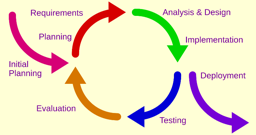
\includegraphics{fig/modelo_incremental}
			 \caption{Modelo incremental}
			 \label{fig:modeloI}
			\end{figure}

			El desarrollo incremental permite desarrollar una parte funcional del proyecto en cada etapa, reservando la mejora o extensión de funcionalidades para el futuro y por tanto controlando la complejidad y los riesgos. Además, este sistema permite a los desarrolladores aprovechar conocimiento adquirido en etapas previas e incorporar nuevo conocimiento y nuevas técnicas en fases venideras.

			Adicionalmente, esta metodología confía en el desarrollo guiado por tests. Esta práctica consiste en el desarrollo de tests antes que código, y después se genera el mínimo código posible para completar esos tests. El objetivo de esta metodología es lograr código limpio y funcional, la idea es que los requisitos se traducen a evidencia, de forma que si los tests se completan satisfactoriamente, se garantiza que el software cubre dicho requisitos.

		\subsection{Tareas principales:}

			El desarrollo de Kingdom of Hatred comprende las siguientes tareas o actividades:

			\subsubsection{Lanzamiento del proyecto}

			\begin{itemize}
				\item \textbf{Organización}

				Actividad mediante la que se define y prepara la planificación, asignación de misiones y el lanzamiento del proyecto y sus sucesivas fases.
				\item \textbf{Seguimiento}

				Realización del seguimiento y control del desarrollo del proyecto, que permita la rápida detención y solución de problemas que puedan dificultar la buena marcha del mismo.
			\end{itemize}

			\subsubsection{Análisis de herramientas y técnicas}

			\begin{itemize}
				\item \textbf{Análisis de herramientas para desarrollo de juegos}
				
				Investigar distintas alternativas que existen para el desarrollo de juegos.

				\item \textbf{Análisis de técnicas de generación procedural}
				Investigar distintos algoritmos de generación procedural que sean adecuados para la generación de niveles.
			\end{itemize}

			\subsubsection{Diseño del juego}

			\begin{itemize}
				\item Diseño del juego
				Crear el documento de desarrollo de juego que definirá cómo será este.
			\end{itemize}

			\subsubsection{Desarrollo del software}

			\begin{itemize}
				\item \textbf{Formación}
				Aprendizaje en la creación de juegos.
				\item \textbf{Diseño}
				Diseño del software del juego.
				\item \textbf{Implementación}
				Implementación del juego.
			\end{itemize}

			\subsubsection{Validación técnica y de usabilidad:}

			\begin{itemize}
				\item \textbf{Betatesting}
				Uso intensivo del juego en busca de bugs.
				\item \textbf{Prueba de experiencia de usuario}
				Recoger opiniones para mejorar la experiencia de usuario.
			\end{itemize}

			\subsubsection{Distribución y cierre del proyecto}

			\begin{itemize}
				\item \textbf{Despliegue de la versión final}
				
				Preparar el juego para el usuario final.
				\item \textbf{Cierre del proyecto}

				Cierre del proyecto.
			\end{itemize}

		\subsection{Productos intermedios:}

			Los productos intermedios que se generarán en cada una de las fases son:

			\begin{itemize}
				\item \textbf{Diseño del juego:}
				\begin{itemize}
					\item Documento de diseño de juego.
				\end{itemize}
				\item \textbf{Desarrollo del software:}
				\begin{itemize}
					\item Documento con la especificación del software.
				\end{itemize}
				\item \textbf{Validación técnica y usabilidad:}
				\begin{itemize}
					\item Informe de evaluación del juego.
				\end{itemize}
			\end{itemize}

	\section{Organización}

		\subsection{Esquema organizativo}

			La organización del proyecto se articula en torno al comité de dirección y al equipo de trabajo que se va a encargar de desarrollar el producto, en función de la estructura de la Figura \ref{fig:esqOrg}.

			\begin{figure}[!htp]
				\centering
				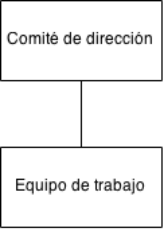
\includegraphics[scale=.75]{fig/esq}
				\caption{Esquema Organizativo}
				\label{fig:esqOrg}
			\end{figure}

			\begin{itemize}
				\item Comité de dirección 
				Su función principal es asesorar el proyecto y la toma de decisiones. Formado por el jefe de proyecto.
				\item Equipo de trabajo
				El órgano encargado de diseñar, desarrollar y testear el contenido del proyecto en función de las diferentes fases estipuladas. Formado por el programador, el diseñador y el tester.
			\end{itemize}

		\subsection{Plan de recursos humanos}

			\label{sec:planRecursosHumanos}

			El equipo de trabajo estará formado por los siguientes perfiles directamente relacionados con las diferentes áreas de competencias que abordan el proyecto:

			\begin{itemize}
				\item Jefe de proyecto:
				Sus funciones son realizar las actividades de organización, coordinación y seguimiento del proyecto. Por otro lado, deberá encargarse del diseño del juego. Con un jefe de proyecto es suficiente. Para el perfil será necesario alguien con experiencia en comunicación interpersonal, liderazgo y solución de problemas.
				\item Programador:
				Encargado de diseñar e implementar el software en base al diseño del 	juego. Será necesario conocimiento de ingeniería del software para llevar a cabo las tareas asignadas a este perfil.
				\item Tester:
				Encargado de probar el producto y reportar errores y sugerir mejoras. 	Para hacer las 	pruebas de fase beta será suficiente con un tester. 	Sin embargo, para las prueba de 	experiencia de usuario sería 	conveniente contar con el mayor número de personas 	posibles. El tester debe ser tener imaginación y ser creativo para llevar al juego a situaciones límite y encontrar el mayor número de errores posible.
			\end{itemize}

	\section{Condiciones de ejecución}

		\subsection{Entorno de trabajo}

			El lugar de trabajo habitual será el domicilio del trabajador.
			El calendario y horario serán 3 horas al día, de lunes a viernes.
			Los medios informáticos para la ejecución corren a cargo del trabajador. Los medios de los que se disponen actualmente y se usarán son los siguientes: 

			\begin{itemize}
				\item Hardware
				\begin{itemize}
					\item Ordenador de sobremesa completo con monitor secundario
					\item Ordenador portátil
				\end{itemize}
				\item Software
				\begin{itemize}
					\item Todo el software que se use será gratuito, así que este apartado no supondrá un problema.
				\end{itemize}
			\end{itemize}

		\subsection{Diálogo durante el proyecto}

			Durante el proyecto y para la correcta marcha del mismo, una comunicación constante entre el comité de dirección del proyecto y el equipo de desarrollo va a ser necesaria, y por tanto realizada. El equipo de desarrollo deberá atender a todas la reuniones para discutir el progreso, las mejoras y los requisitos del proyecto.

		\subsection{Recepción de productos}

			Los productos generados durante el proyecto son el punto de partida para trabajo venidero, y deben ser enviados al jefe de proyecto para evaluación y aprobado.

			Tras el envío, habrá 3 días laborables para comunicar cualquier error o comentario al equipo de trabajo, el cual procederá a crear una revisión del documento y comenzará un nuevo periodo de aprobación. Si pasados los 3 días laborables no se ha recibido respuesta, la entrega se considerará válida.

			Durante el desarrollo de cualquiera de los productos del proyecto, el jefe de proyecto asume 	la responsabilidad si cualquiera de ellos no se hace o no alcanza la calidad esperada. 	Consecuentemente, el jefe de proyecto debe cercionarse que el trabajo de todos marcha 	adecuadamente y tomar medidas correctoras en caso contrario.

			El jefe de proyecto será el portavoz del equipo de desarrollo durante la marcha del proyecto, 	y tendrá que comunicarse con el tutor e informarle adecuadamente del estado de la 	realización en cada momento.

		\subsection{Control de cambios}

			Tanto jefe de proyecto como el tutor tienen potestad para pedir modificaciones en las 	especificaciones, diseños o desarrollos ya realizados. En caso de querer modificar algo, se 	seguirá el siguiente procedimiento:

			\begin{enumerate}
				\item Comunicación formal del solicitante de las modificaciones solicitadas.
				\item Valoración, por parte del jefe del proyecto y el equipo de desarrollo, de la repercusión 	técnica, económica y el plazo de ejecución.
				\item Presentación de una propuesta valorada al solicitante.
				\item Notificación, por parte del solicitante, de la aprobación o no de la propuesta.
				\item En caso afirmativo, modificación del plan de trabajo y presupuesto.
			\end{enumerate}

	\section{Planificación}

		\subsection{Plan de trabajo}

			\begin{figure}[!htp]
				\centering
				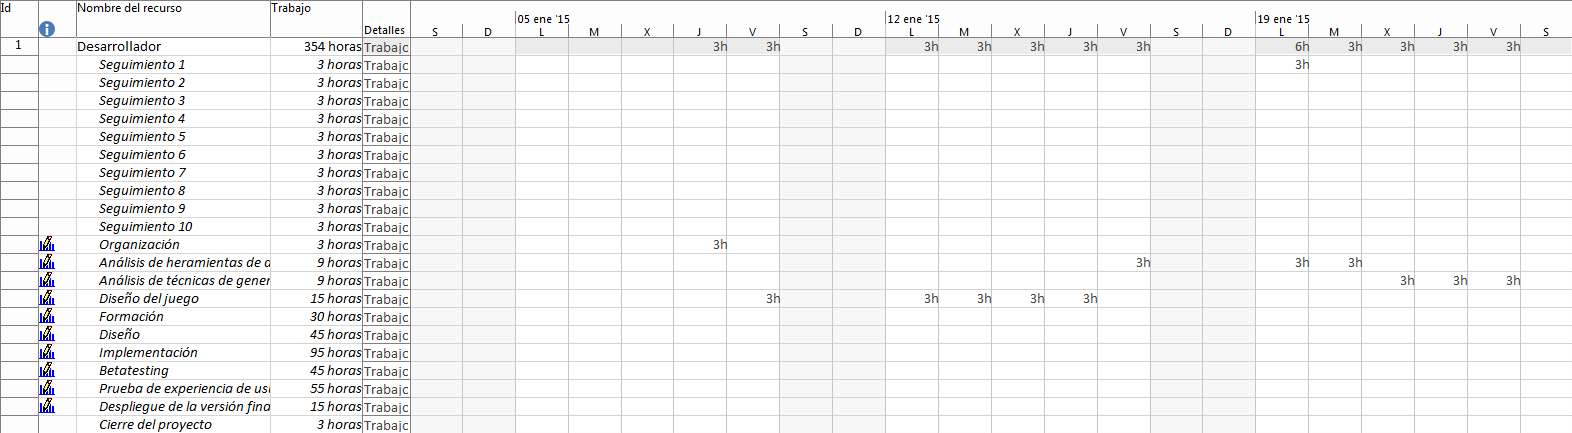
\includegraphics[page=1, scale=.5, angle=90]{fig/Plan1}
				\caption{Diagrama del plan de trabajo 1}
			\end{figure}

			\begin{figure}[!htp]
				\centering
				\includegraphics[page=2, scale=.5, angle=90]{fig/Plan2}
				\caption{Diagrama del plan de trabajo 2}
			\end{figure}

			\begin{figure}[!htp]
				\centering
				\includegraphics[page=3, scale=.5, angle=90]{fig/Plan3}
				\caption{Diagrama del plan de trabajo 3}
			\end{figure}

			\begin{figure}[!htp]
				\centering
				\includegraphics[page=4, scale=.5, angle=90]{fig/Plan4}
				\caption{Diagrama del plan de trabajo 4}
			\end{figure}

			\begin{figure}[!htp]
				\centering
				\includegraphics[page=5, scale=.5, angle=90]{fig/Plan5}
				\caption{Diagrama del plan de trabajo 5}
			\end{figure}

			\begin{figure}[!htp]
				\centering
				\includegraphics[page=6, scale=.5, angle=90]{fig/Plan6}
				\caption{Diagrama del plan de trabajo 6}
			\end{figure}

			\begin{figure}[!htp]
				\centering
				\includegraphics[page=7, scale=.5, angle=90]{fig/Plan7}
				\caption{Diagrama del plan de trabajo 7}
			\end{figure}

			\begin{figure}[!htp]
				\centering
				\includegraphics[page=8, scale=.5, angle=90]{fig/Plan8}
				\caption{Diagrama del plan de trabajo 8}
			\end{figure}

			\FloatBarrier

		\subsection{Diagrama de Gantt}
			\begin{figure}[!htp]
				\centering
				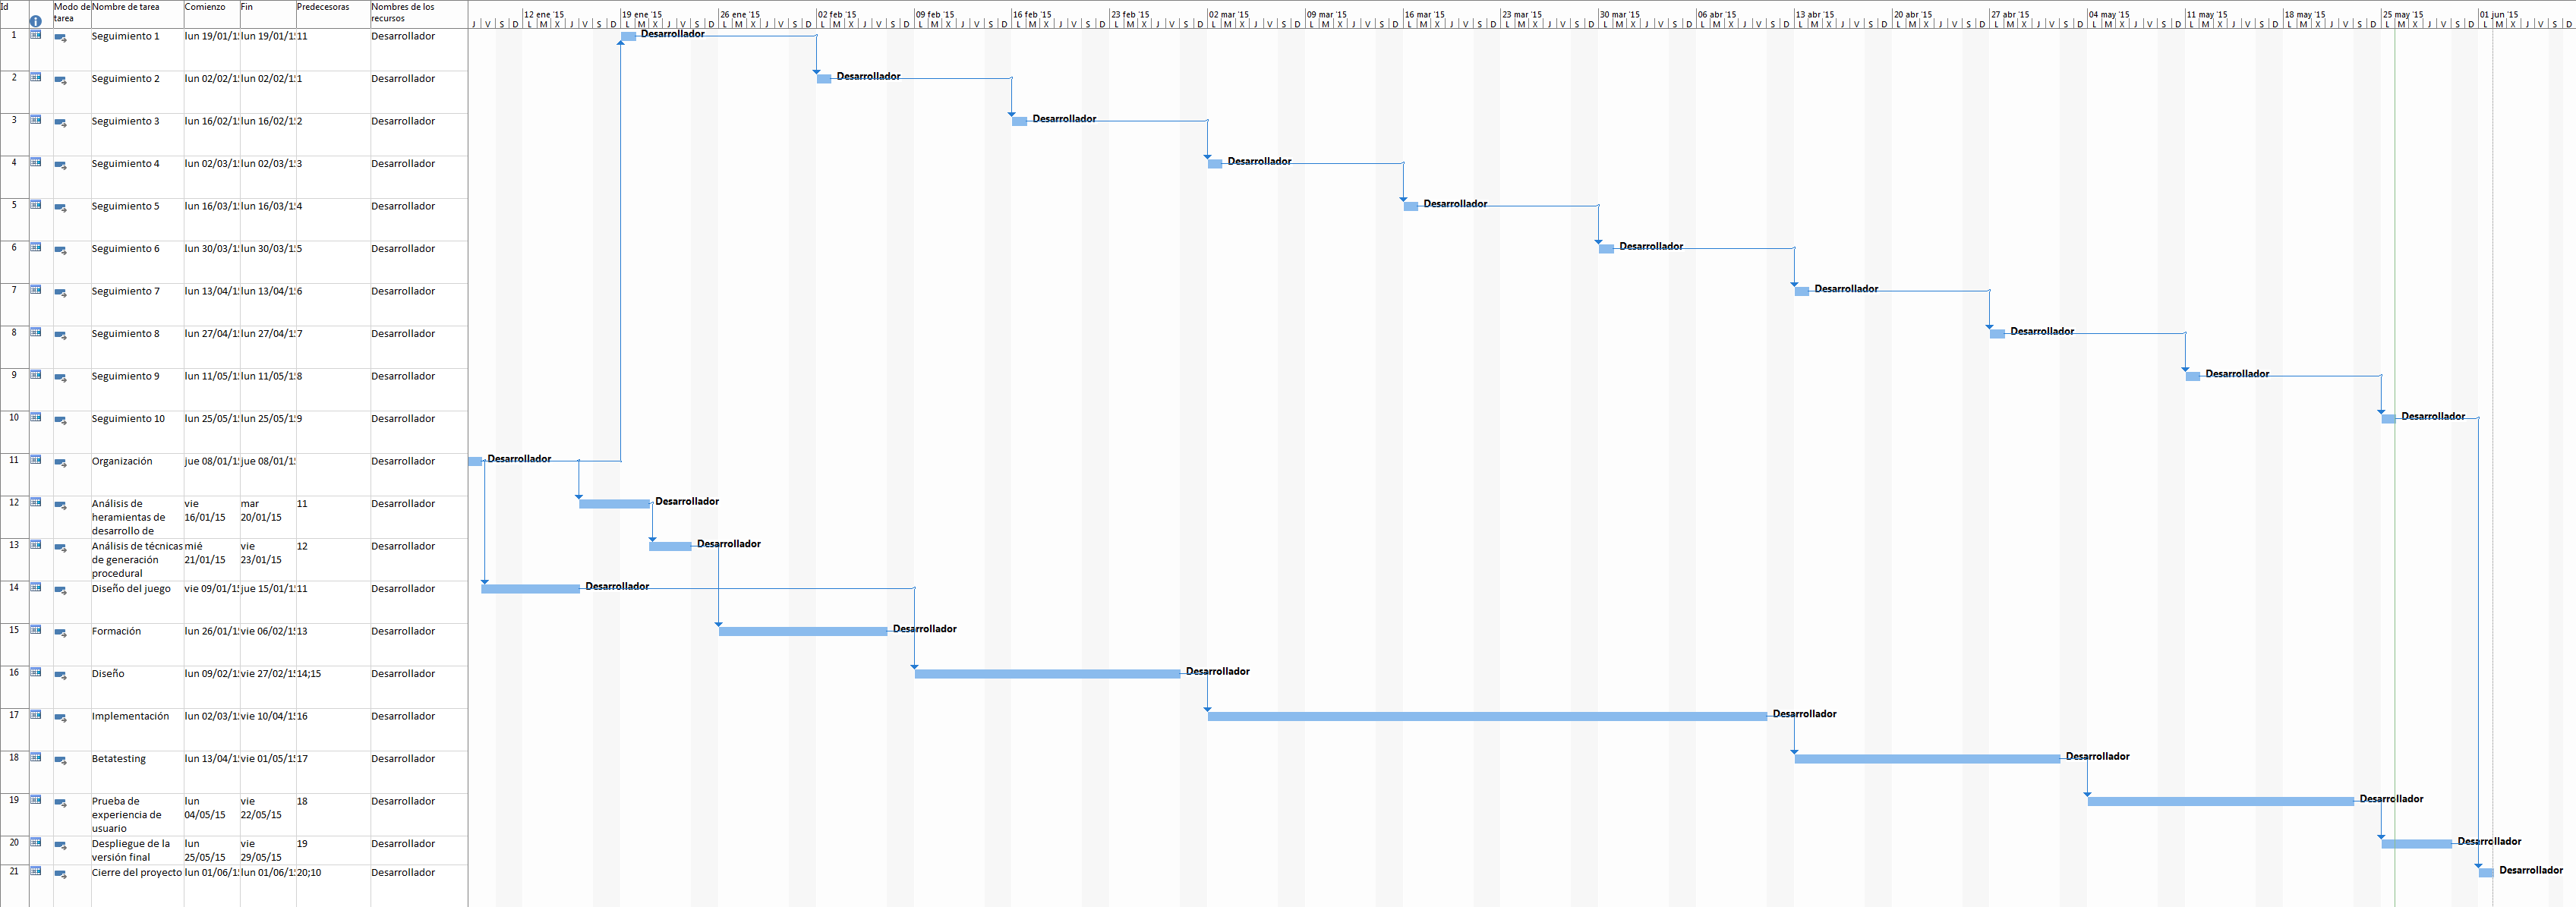
\includegraphics[page=1, scale=.25, angle=90]{fig/Gantt}
				\caption{Diagrama de Gantt}
			\end{figure}

			\FloatBarrier

		\subsection{Diagrama de Red}
			\begin{figure}[!htbp]
				\centering
				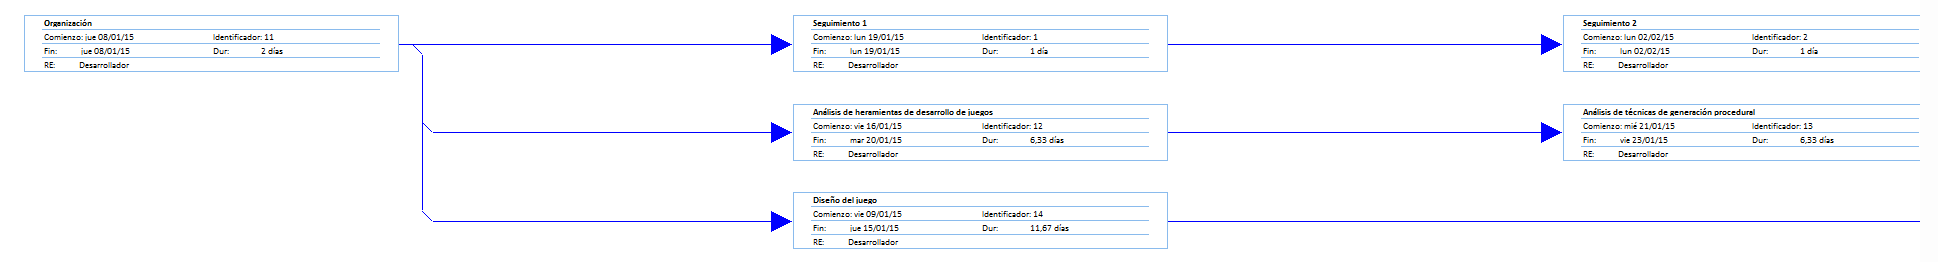
\includegraphics[scale=.4, angle=90]{fig/Red1}
				\caption{Diagrama de precedencias 1}
			\end{figure}

			\begin{figure}[!htbp]
				\centering
				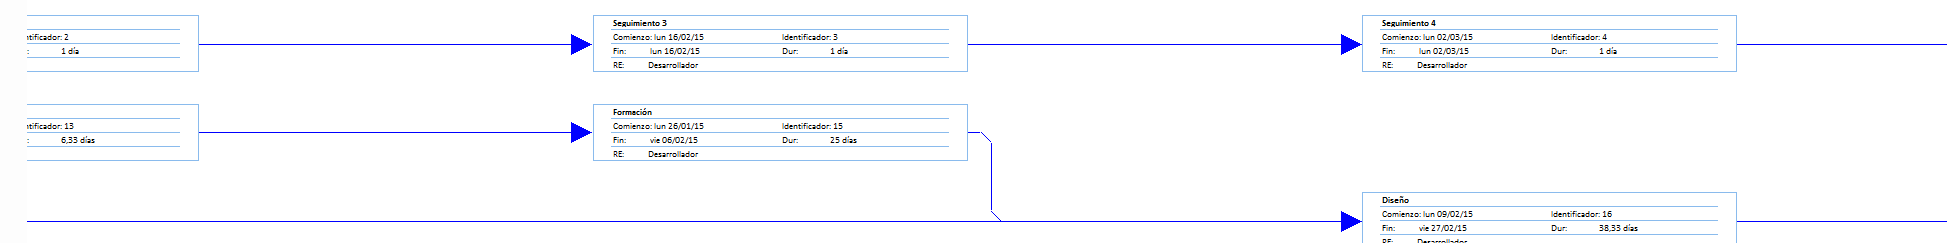
\includegraphics[scale=.4, angle=90]{fig/Red2}
				\caption{Diagrama de precedencias 2}
			\end{figure}

			\begin{figure}[!htbp]
				\centering
				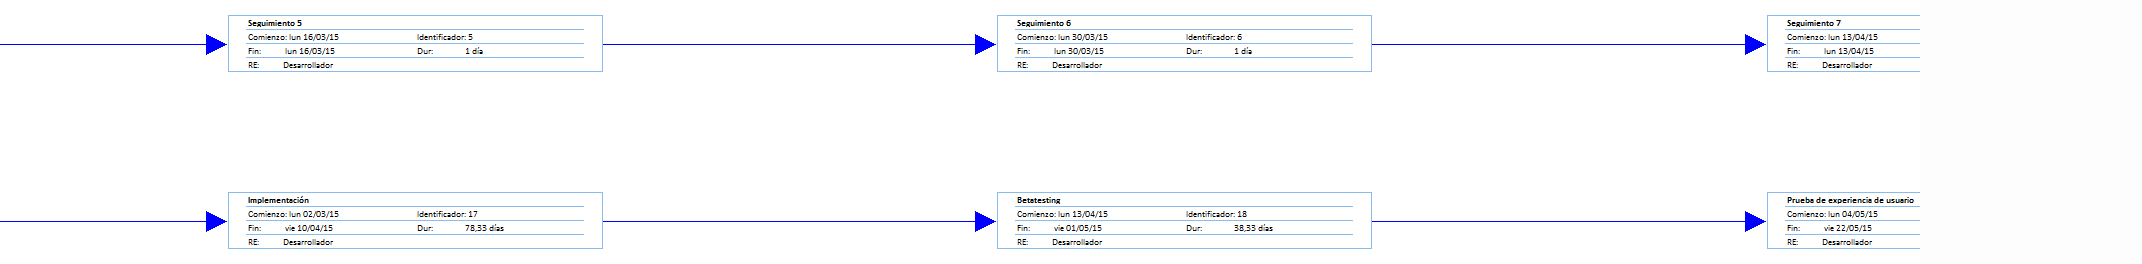
\includegraphics[scale=.4, angle=90]{fig/Red3}
				\caption{Diagrama de precedencias 3}
			\end{figure}

			\begin{figure}[!htbp]
				\centering
				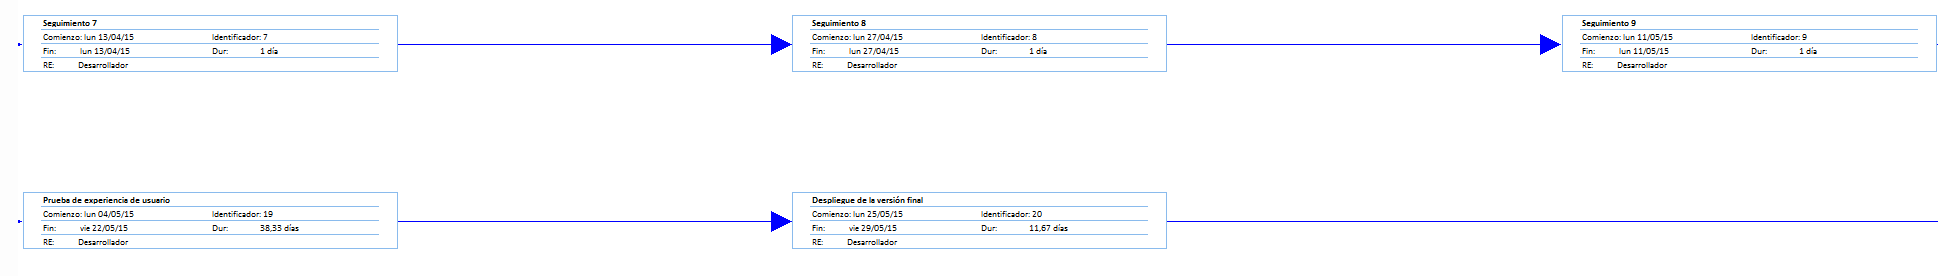
\includegraphics[scale=.4, angle=90]{fig/Red4}
				\caption{Diagrama de precedencias 4}
			\end{figure}

			\begin{figure}[!htbp]
				\centering
				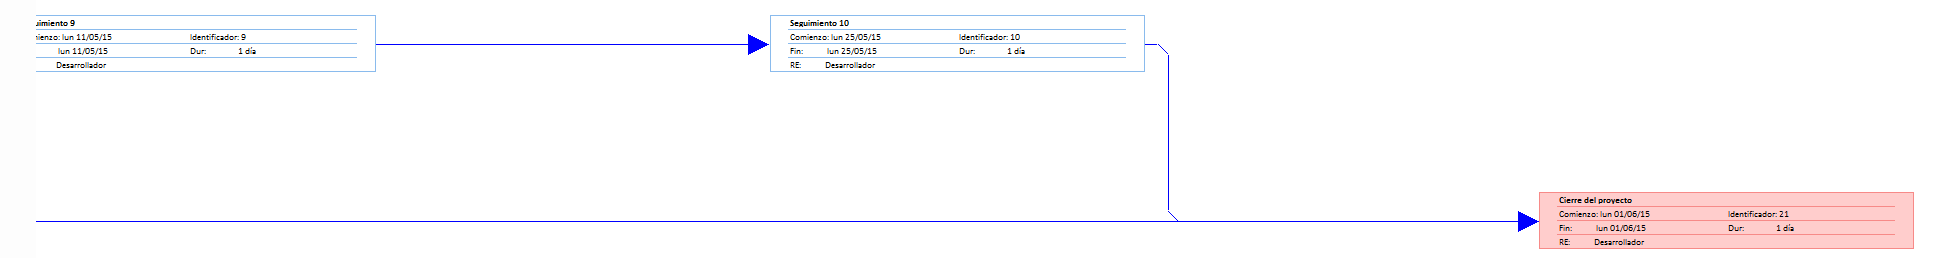
\includegraphics[scale=.4, angle=90]{fig/Red5}
				\caption{Diagrama de precedencias 5}
			\end{figure}

			\FloatBarrier

	\section{Presupuesto}

		\subsection{Software}

			Todas las herramientas utilizadas para la realización del proyecto han sido de código abierto o gratuitas, de forma que el coste derivado de la adquisición de productos o servicios software es nulo.

		\subsection{Hardware}

			\begin{center}
				\captionof{table}{Presupuesto: Hardware}
				\begin{tabular}{| l | r | r | r |}
					\hline
					Nombre				&	Precio(\euro)	&	Unidades	&	Importe total(\euro)	\\	\hline
					Ordenador de sobremesa			& 	1500			&	1 			&	1500					\\	\hline
					Ordenador portátil	&	700				&	1			&	700						\\
					\hline
				\end{tabular}
			\end{center}

		\subsection{Recursos humanos}

			\begin{center}
				\captionof{table}{Presupuesto: Recursos Humanos}
				\begin{tabular}{| l | r | r | r |}
					\hline
					Rol					&	Precio/hora(\euro/h)	&	Carga de trabajo(h)	&	Importe total(\euro)	\\	\hline
					Jefe de proyecto	& 	30						&	54 					& 	1620,00				\\	\hline
					Programador			&	25						&	321					&	8025,00			\\	\hline
					Tester			&	15						&	90					&	1350,00				\\	\hline
				\end{tabular}
			\end{center}

		\subsection{Total}

			\begin{center}
				\captionof{table}{Presupuesto: Total}
				\begin{tabular}{| l | r |}
					\hline
					Tipo				&	Total			\\	\hline
					Recursos Humanos	& 	10995		\\	\hline
					Recursos Hardware	&	2200		\\	\hline
					\textbf{Total}		&	\textbf{13195}	\\
					\hline
				\end{tabular}
			\end{center}
